\graphicspath{
    {figures_and_references/urban_surface_detection/}
    {figures_and_references/EELISA_conference/}
    {figures_and_references/footprints_paper/}
}

% \selectlanguage{english}
\renewcommand{\chapternametext}{Chapter \thechapter . Use case: Machine learning-based classification of structural systems from remote sensing attributes in the 3 pilot regions}
\renewcommand{\shortchapternametext}{Chapter \thechapter . Use case: Structural system classification}

\begin{refsection}

\chapter{\chapternametext}
\

\renewcommand{\headingtextL}{}
\renewcommand{\headingtextR}{\shortchapternametext}
\begingroup
 \flushbottom
 \setlength{\parskip}{0pt plus 1fil}%
 \localtableofcontents 
\endgroup

\begingroup
 \flushbottom
 \setlength{\parskip}{0pt plus 1fil}%
 \locallistoffigures
 \locallistoftables
\endgroup


\newpage

\setcounter{section}{0} 



\FloatBarrier

\renewcommand{\sectionnametext}{Experimental setup}
\renewcommand{\headingtextL}{\shortchapternametext}
\renewcommand{\headingtextR}{\thesection. \sectionnametext}
\section{\sectionnametext}

Three structural systems are the majority present in the dataset (fig. \ref{fig:structural_material_survey}) and are considered meaningful enough for training: masonry [M], concrete [CR] and adobe [M99/ADO]. Several classification models have been employed to evaluate performance on an imbalanced dataset, where the minority class is \textit{M99/ADO}. To address the imbalance, two approaches have been utilized: using class weights during training and applying the oversampling technique SMOTE. 

\renewcommand{\sectionnametext}{Results}
\renewcommand{\headingtextR}{\thesection. \sectionnametext}
\section{\sectionnametext}

The classification models tested include a multinomial logistic regression classifier (LR) \footcite{bishop_pattern_2016}, XGBoost \footcite{Chen:2016btl}, Random Forest (RF) \footcite{parmar_review_2019} and TabPFN \footcite{hollmann_accurate_2025, hollmann_tabpfn_2023}, a foundation model for tabular data. The best performance comes from the simplest model, the logistic regression model.

\begin{table}[ht]
\centering
\begin{tabular}{l|c|ccc|cc}
\toprule
\textbf{Model} & \textbf{Acc} & \multicolumn{3}{c}{\textbf{F1 Score (per class)}} & \multicolumn{2}{c}{\textbf{Weighted Avg}} \\ 
& & \textbf{CR} & \textbf{M} & \textbf{M99/ADO} & \textbf{Recall} & \textbf{F1 Score} \\
\midrule
LR & 0.87 & 0.80 & 0.84 & 0.95 & 0.87 & 0.87 \\
LR (SMOTE) & 0.87 & 0.80 & 0.84 & 0.96 & 0.87 & 0.87 \\
RF & 0.74 & 0.74 & 0.73 & 0.76 & 0.74 & 0.75 \\
RF (SMOTE) & 0.84 & 0.78 & 0.81 & 0.92 & 0.84 & 0.84 \\
XGBoost & 0.83 & 0.75 & 0.80 & 0.93 & 0.83 & 0.83 \\
XGBoost (SMOTE) & 0.83 & 0.76 & 0.80 & 0.92 & 0.83 & 0.83 \\
TabPFN & 0.86 & 0.75 & 0.84 & 0.96 & 0.86 & 0.85 \\
\bottomrule
\end{tabular}
\caption{Performance comparison of classification models on an imbalanced dataset. CR: Concrete, M: Masonry, M99/ADO: Adobe.}
\label{tab:comparison}
\end{table}

\begin{figure}[htbp]
    \centering
    \begin{tabular}{ccc}
        \begin{subfigure}[t]{0.3\linewidth}
            \centering
            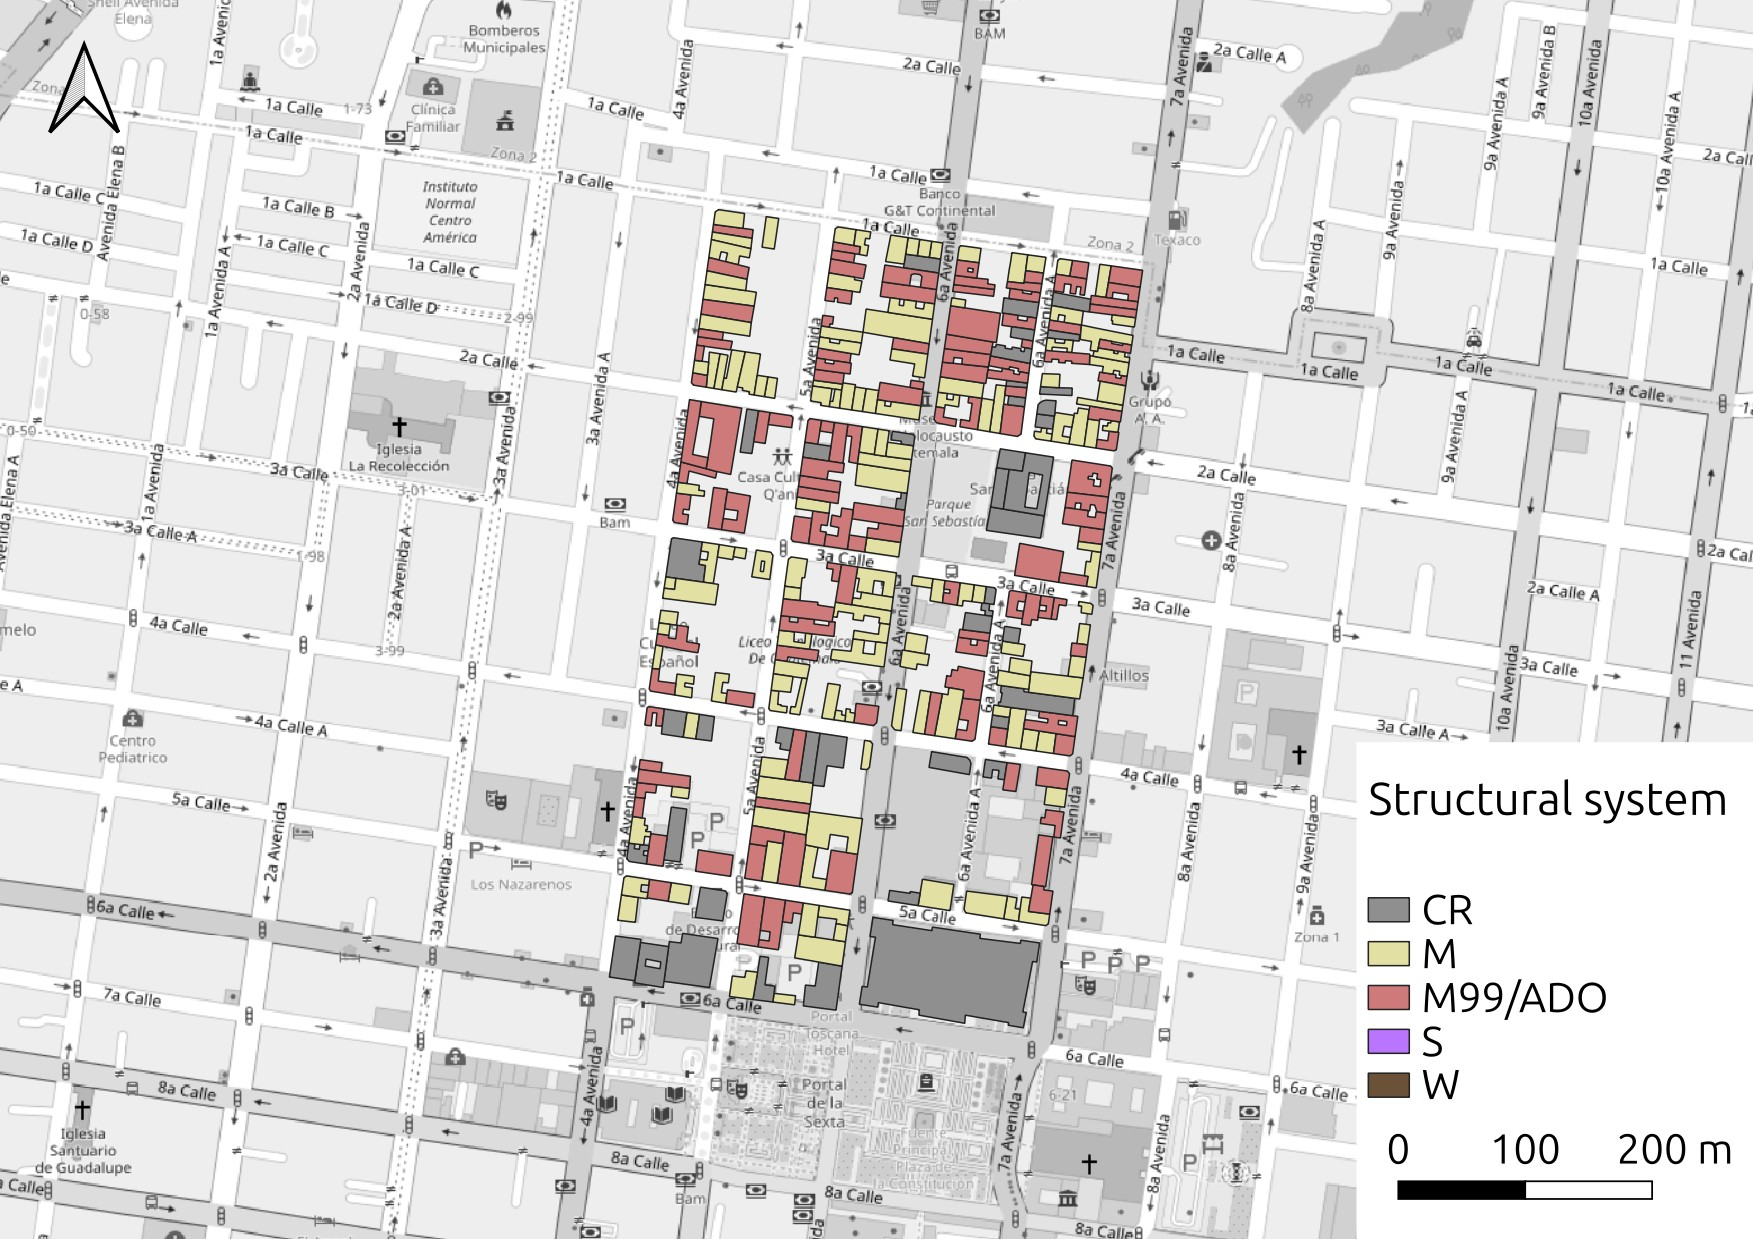
\includegraphics[width=\linewidth]{figures/structural_system_Guatemala.jpg}
            \caption{Ciudad de Guatemala (Guatemala)}
        \end{subfigure} & 
        \begin{subfigure}[t]{0.3\linewidth}
            \centering
            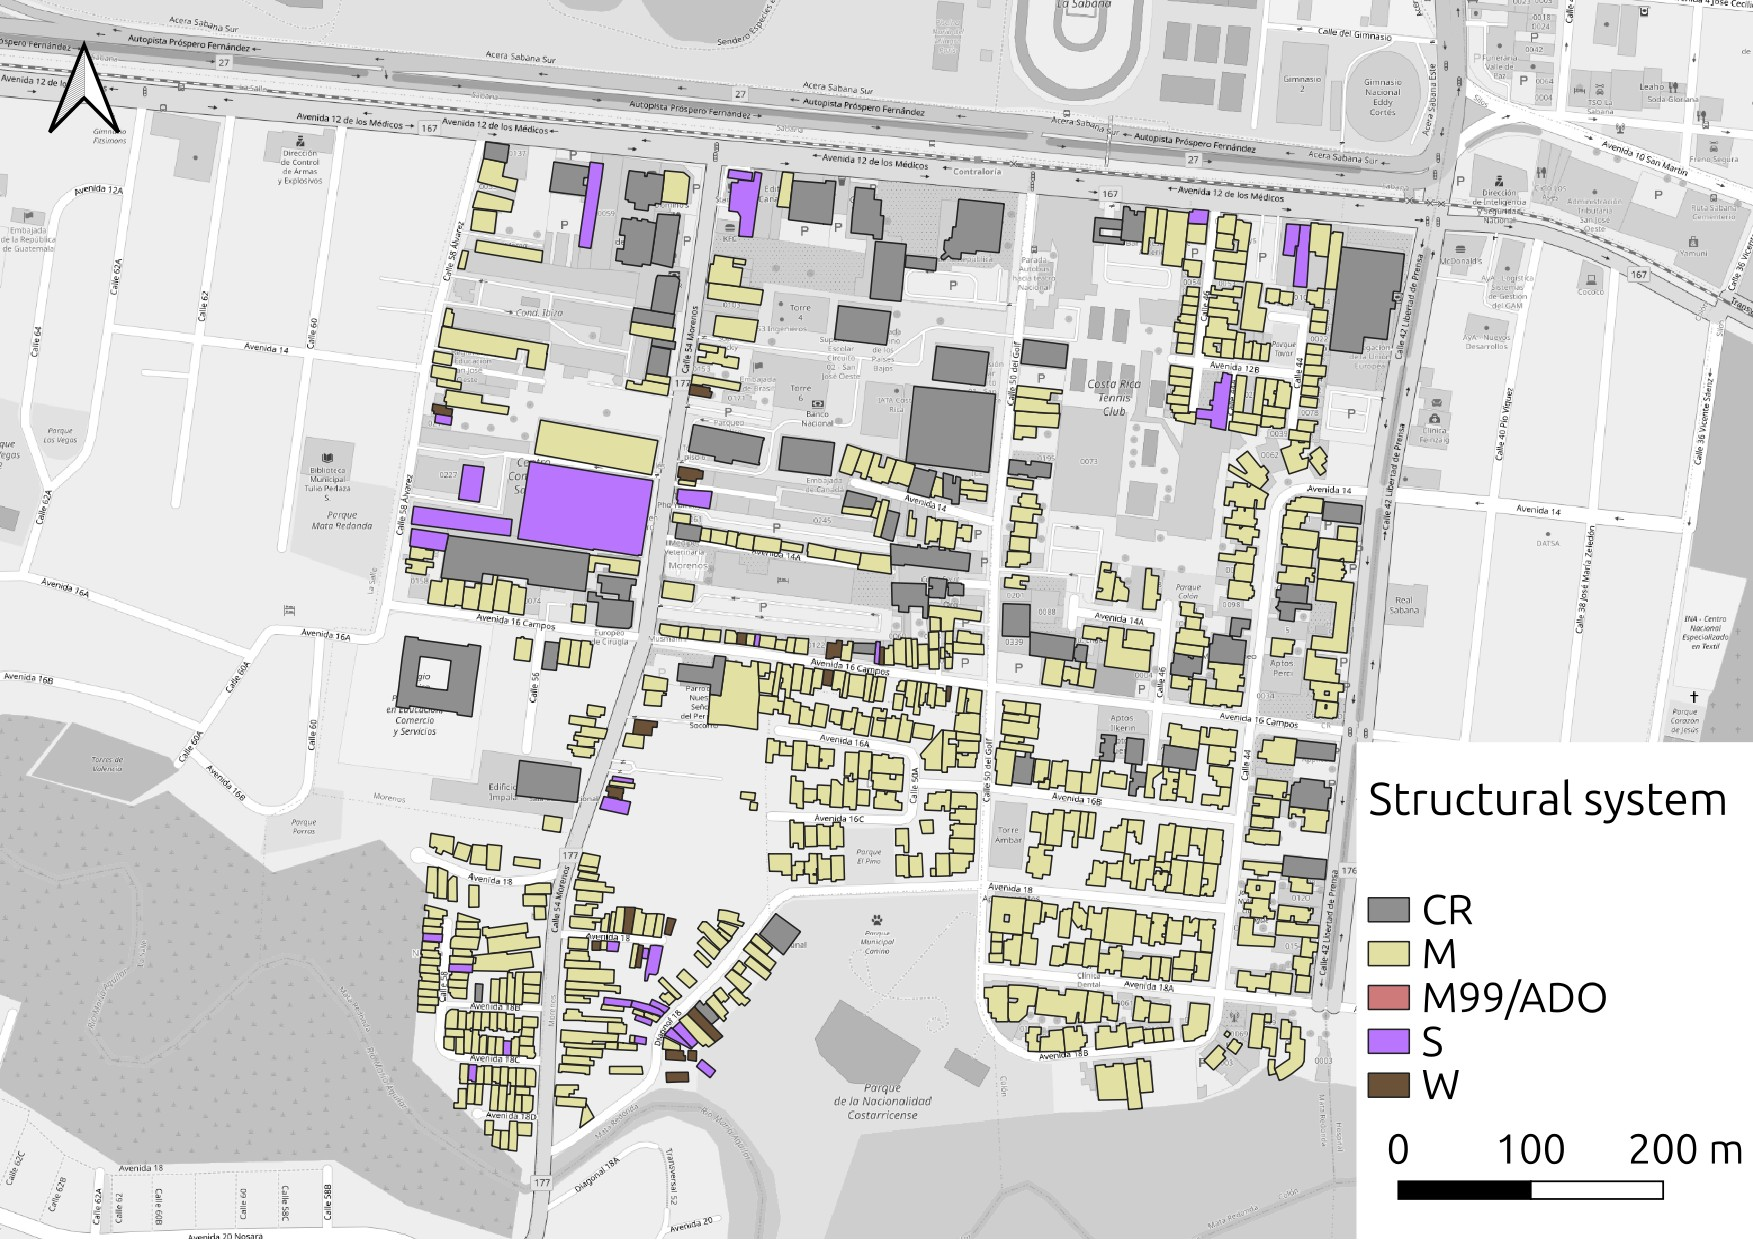
\includegraphics[width=\linewidth]{figures/structural_system_San José.jpg}
            \caption{San Jośe (Costa Rica)}
        \end{subfigure}  & 
        \begin{subfigure}[t]{0.3\linewidth}
            \centering
            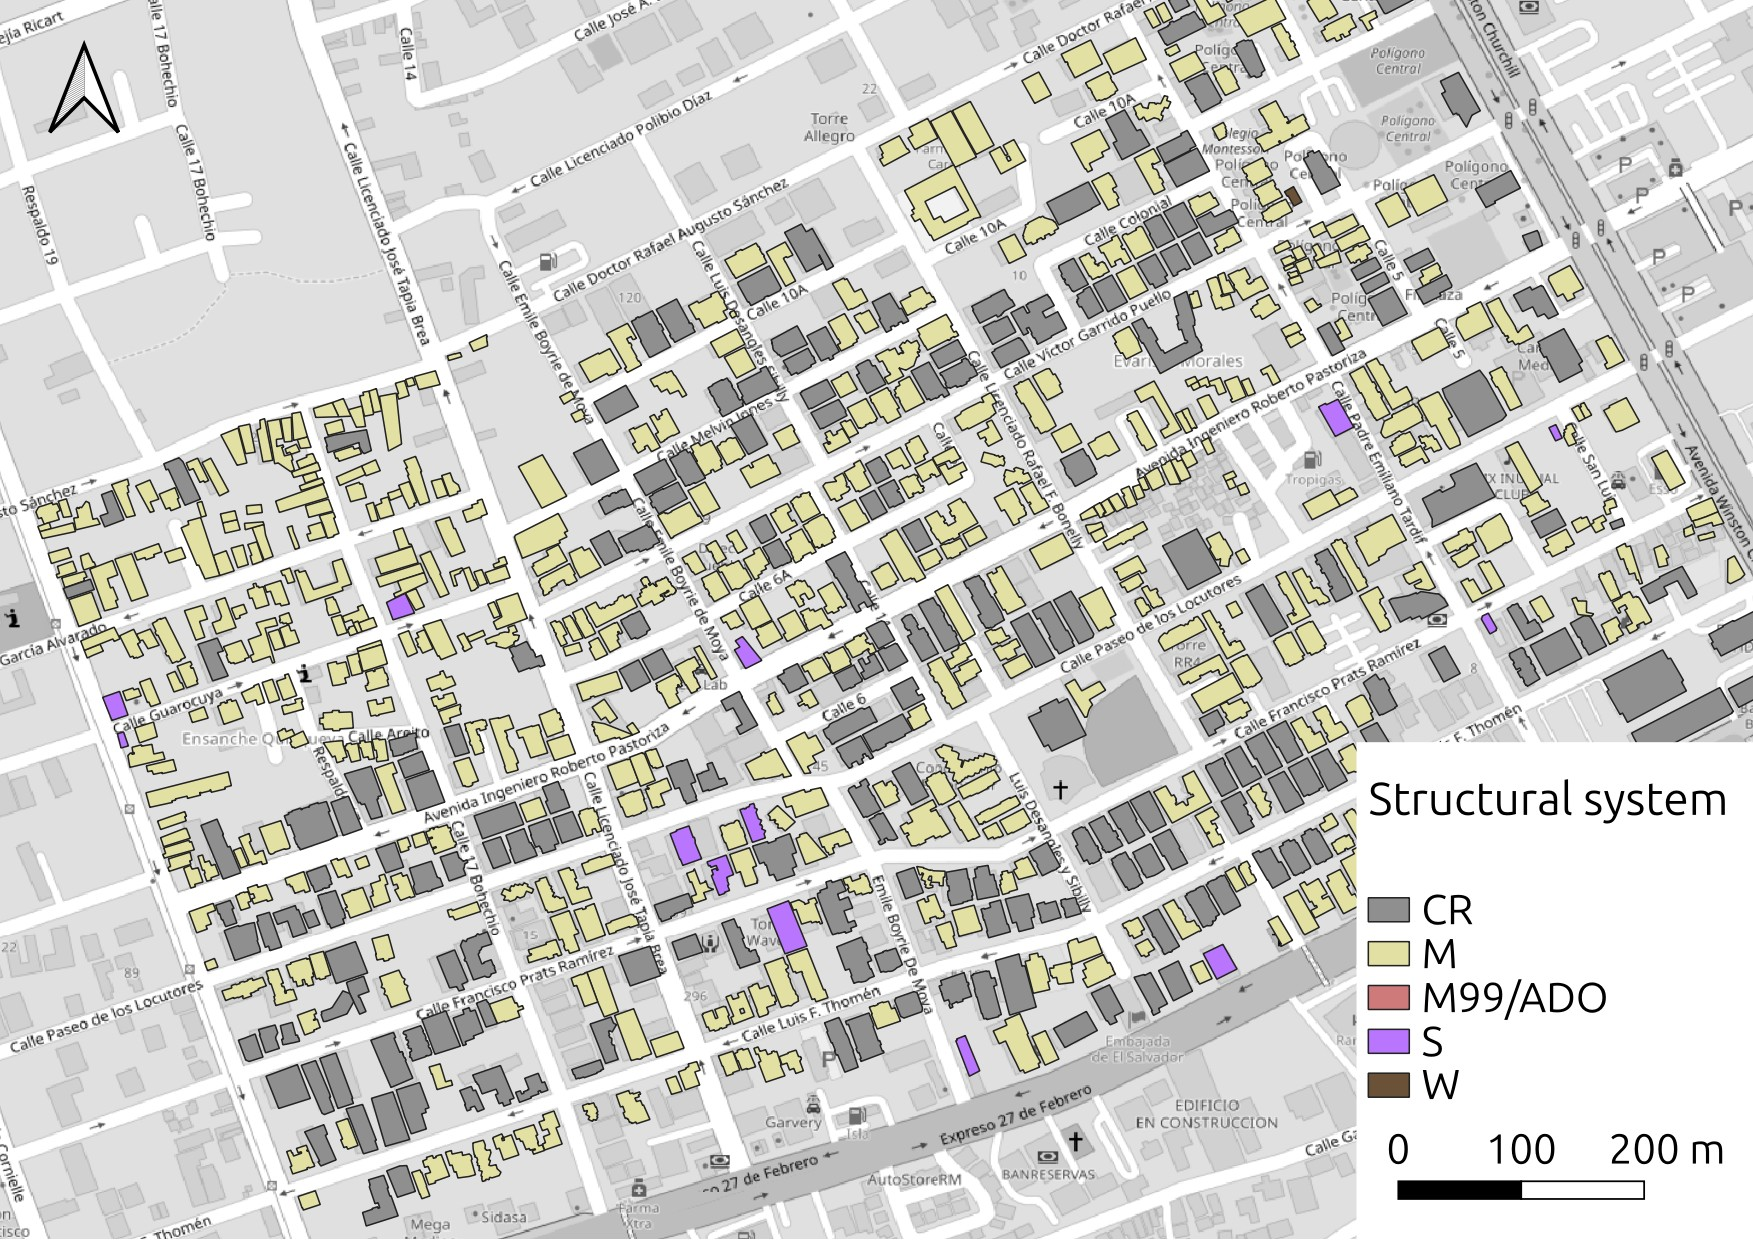
\includegraphics[width=\linewidth]{figures/structural_system_Santo Domingo.jpg}
            \caption{Santo Domingo (Dominican Republic)}
        \end{subfigure} 
    \end{tabular}
    \caption{Structural system according to the field survey in the three pilot regions.}
    \label{fig:structural_material_survey}
\end{figure}


\newpage

\renewcommand{\sectionnametext}{References}
\renewcommand{\headingtextR}{\thesection. \sectionnametext}
\section{\sectionnametext}
\printbibliography[heading=none]

\end{refsection}